% !TeX root = ../main.tex
\chapter{Installation}
\section{Introduction}
In this chapter, we will install and complete the installation of HobbySpark and all of its dependencies.
You will need an internet connection and enough space for the app to be installed (Do not worry about disk space, HobbySpark is in mere megabytes). 

\section{Installing HobbySpark}
\begin{notebox}
	HobbySpark is supported currently for all the 3 mainstream operating systems-- Windows, Debian Linux, and MacOS. However, this documentation explains the installation procedure for windows only.
	\begin{itemize}
		\item The Linux install procedure is quite straight-forward, which you can easily follow.
		\item MacOS may be a bit trickier though, as HobbySpark is an open-source application. A open-source app can be licensed and notorised by Apple. Hoever, we haven't licensed and notorised  our app. However, you can follow the website's FAQ page and there will be instructions for how to install the app for MacOS 
	\end{itemize}
\end{notebox}

First, visit \href{https://sites.google.com/view/hobbyspark/downloads/windows}{here} and go down to the installer download button. Click the button. Once the download is finished, run the installer.

Now, you should probably see something close to Fig~\ref{fig:bsod}. {\Large Do not panic}, this is normal behavior, as HobbySpark does not have a software license from microsoft. Therefore, Windows does not know that there is an app called this, so it warns you that ithas an unverified publisher. As long as the app is from the real genuine repo or the genuine website, it's safe to press \code{more info} and then \code{run anyway}.
\begin{figure}[H]
	\centering
	\caption{The windows smart-screen}
	\label{fig:bsod}
	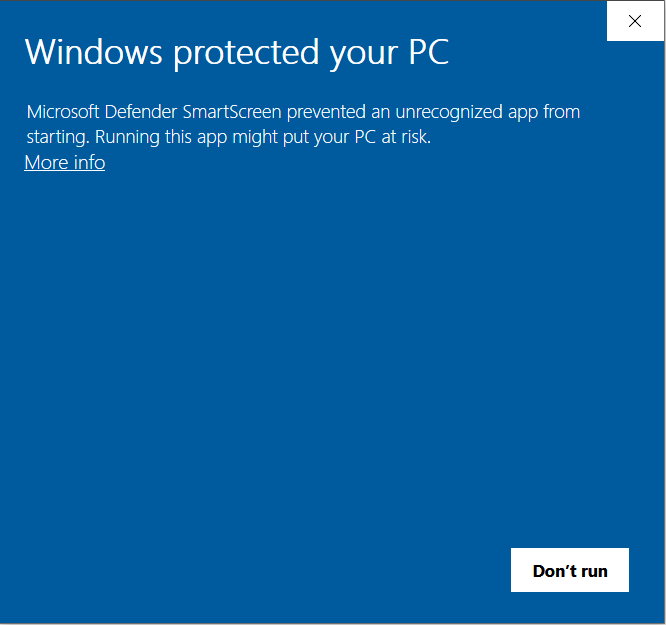
\includegraphics[scale=0.3]{images/bsod.png}
\end{figure}
\newpage
\subsection{Starting it up}
Now, once you click \code{run anyway}, the installer will ask you to choose the language for the installation process\emph{only}, so the app will be in English no matter what language you choose for installation.

\subsection{License agreement}
Now a license agreement page will show up. For your information, HobbySpark uses the Apache version 2.0 license. For those who don't know about it are free to read it. After doing that, click \code{I accept the agreement}.

\subsection{Important info and additional steps}
Now, it'll show you what you can do with HobbySpark as a short introduction. Next, it shows a window with a checkbox. You can check it if you want a desktop shortcut for HobbySpark.

\subsection{Actual installation}
Now it'll show you the various settings you have chosen, which should be similar to--
\begin{lstlisting}[style=tracebacks]
	Additional tasks:
	Additional shortcuts:
	Create a desktop shortcut
\end{lstlisting}


Next, you can press install. You will see a progress-bar. You can be sure the installation is almost finished when language names start appearing above the progress-bar. Next press finish and optionally check \code{Launch} to open HobbySpark immediately. 
\section{After installation}
Depending on whether you have some apps or not, you may or may not get a window to install Python and Arduino-cli. If these show up, follow the steps on the screen. Also, it may take a few moments for the app to open the first time as it installs some dependencies internally.

The first time you check or upload, it may pop up with a window saying that HobbySpark is installing some dependencies. These are Arduino frameworks. Please wait until the installation is complete. 

An internet connection will be required when you open the app for the first time, even if through the installer, or it may even end you up with an error.